\chapter{Umsetzung des neuronalen Netzes zur Erkennung von Interaktionen}
Im Rahmen des Praxisprojekts entstand ein Prototyp, welcher ein Sofa darstellt, dass als Steuerung für smarte Endgeräte dient. Verwaltet wird das ganze von einem Regelsystem, welches nun durch ein neuronales Netz werden soll. Das aktuelle Kapitel erläutert die Umsetzung von der Aufgabe eines neuronalen Netzes im Smart Home bis zu den Funktionen des neuronalen Netz zur Verwaltung der Interaktionen.

\section{Umsetzung des neuronalen Netzes in Python}
\label{sec:ums_nn}
Das folgende Kapitel beschreibt die Umsetzung des neuronalen Netzes ohne eine Machine Learning Bibliothek und mit einer Bibliothek. Die Vorgehensweise eine Python-Bibliothek für Machine Learning zu nutzen, ist erst nach der Datensammlung mit verschiedenen Probanden kam erst als spätere Erkenntnis. Da der Datensatz sehr groß ist und die Nutzung einer schon vorhanden Bibliothek daher ein Vorteil ist um einfache Änderungen zur besseren Vorhersage vornehmen zu können.

\subsection{Umsetzung des neuronalen Netzes mit Numpy}


\subsection{Umsetzung des neuronalen Netzes mit Keras}
Das neuronale Netz bedient sich zur Umsetzung dem Frontend Keras. Dies ist eine unterstützte Bibliothek von Tensorflow. Tensorflow ist das backend und damit führt Keras alle Berechnungen und Vorhersagen durch. Da Keras eine Bibliothek für Python ist, ist das neuronale Netz auch entsprechende damit umgesetzt.
\newline
Als Ergänzung zu der Erklärung aus den Grundlagen \ref{sec:NNK} ist noch erweitert zu erläutern, dass das neuronale Netz zum Training in diesem Projekt Datensätze aus einer CSV-Dateien einliest. Die Testdaten werden aus dem Dataset als zufällige Anzahl ausgewählt. 
\newline
Das Fully-connected Neural Network ist untereinander mit allen Schichten verbunden. Zu Beginn muss ein Sequential Objekt in Python deklariert werden, damit das neuronale Netz Schicht für Schicht aufgebaut werden kann. Als Aktivierungsfunktion der Input Layers wird die ReLU-Funktion (Rectifier Linear Unit) benutzt. Bei dieser Funktion werden Ergebnisse kleiner null mit null ausgegeben und alles darüber mit dem Ergebnis, welches größer null ist. Die Aktivierungsfunktion des Output Layers ist die sigmoid Funktion. Als Fehlerfunktion wird Mean Squared Error verwendet und Adam als optimizer.
\newline
Aus den versuchen heraus die Fehlerrate zu gering wie möglich zu halten, ist der mittlere quadratische Fehler und die learning rate von 0,001 die beste Wahl.
Die Umsetzung des neuronalen Netzes ist aus einer Vorlage aus dem Buch \citep{frochte2018} entnommen und auf den Trainingsdatensatz vom Sofaprototypen angepasst.


\begin{figure}[H]
	\centering
		%[natürliche Breite in Pixeln, natürliche Höhe in Pixeln, Abhängigkeit von der Textbreite]
		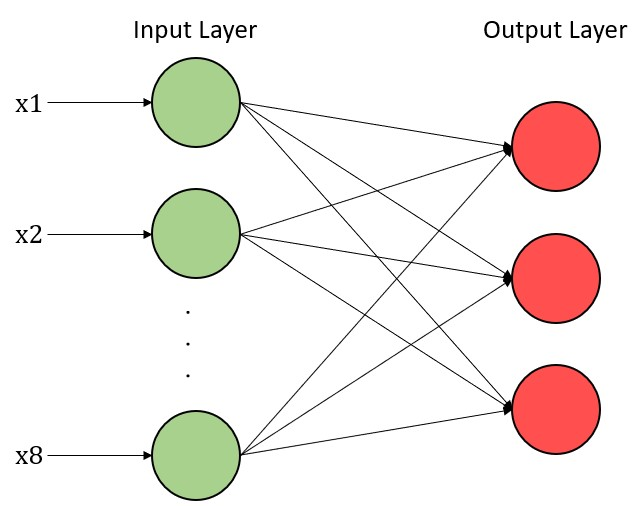
\includegraphics[width=0.6\textwidth]{images/NN.jpg}
	\caption{Darstellung des neuronalen Netzes zur Verwaltung der Interaktionen}
	\label{fig:NN}
\end{figure}

\section{Automatische Erkennung von Interaktionen}
Die Erkennung von Interaktionen findet über die Klassifizierung des neuronalen Netzes statt. Anhand der Ergebnisse aus dem feed forward Schritt und der darauf folgenden Backpropagation findet das neuronale Netz heraus, wie der Nutzer mit dem Sofa interagiert. 
\newline
Kann das neuronale Netz die Vorhersage richtig ausgeben, wird es als Künstliche Intelligenz in den Prototypen aufgenommen. Damit wird dann automatisch erkannt ohne weiteren Einfluss vom Nutzer, welches Gerät gesteuert werden muss.

\section{Neue Funktionen durch das neuronale Netz}
Die Hauptmerkmale zur Erkennung der Interaktionen verändern sich nicht mit dem neuronalen Netz. Das Regelsystem bestimmt anhand der Werte der Sensoren, welche Position der Nutzer auf dem Sofa einnimmt. Dies funktioniert aber nur, wenn die Personen immer für die Positionen die gleichen Sensoren besetzen. So muss für die Sitzposition immer die gleiche Position auf dem Sofa eingenommen werden. Dies ändert sich mit dem neuronalen Netz. Durch die Trainingsdaten wird im neuronalen Netz immer eingelesen wann eine Person sitzt, egal wie sie auf dem Sofa sitzt. Das hat den Effekt, dass jede Person selber entscheiden kann, wie sie sich auf das Sofa setzen möchte. Dadurch kann trotzdem immer das gleiche Endgerät aktiviert werden. Zudem muss bei neuen Liegepositionen und Sitzpositionen keine neue Regel hinzugefügt werden, da das neuronale Netz dies auch erkennent.
\newline
Für die Liegepositionen werden mit dem Regelsystem auch eigene Sensoren verwendet, damit unterschieden werden kann, was auf dem FSR und was mit FlexSensor passiert. Das neuronale Netz kann durch das Training erkennen, wann eine Person mit dem FSR interagiert und sitzt oder liegt. Also wird auf den Sitzkissen nur noch ein Sensor benötigt. Zudem ist es mit FlexSensoren sehr schwer zu erkennen, wann eine Person mit ihm interagiert, da dieser erst den Widerstand ab einer 45 Grad Biegung messen kann.
